\chapter{Экспериментальный раздел}
Техническихе характеристики компьютера, на котором проводились эксперименты.
\begin{itemize}
	\item Операционная система - Windows 10, 64-bit;
	\item Оперативная память - 16 GiB;
	\item Процессор - Intel(R) Core(TM) i7-9750H CPU @ 2.60GHz 2.59 GHz, 6 ядер, 12 потоков.
\end{itemize}

\section{Тестирование работы программы}
В данном подразделе описывается системное тестирование разработанного программного обеспечения. При загрузке программного обеспечения открывается окно, содержащее интерфейс работы с моделью и экран с изображённым на нём кубом. Вид окна приведён ниже на рисунке \ref{fig:qt_test_1}.
\begin{figure}[H]
	\center{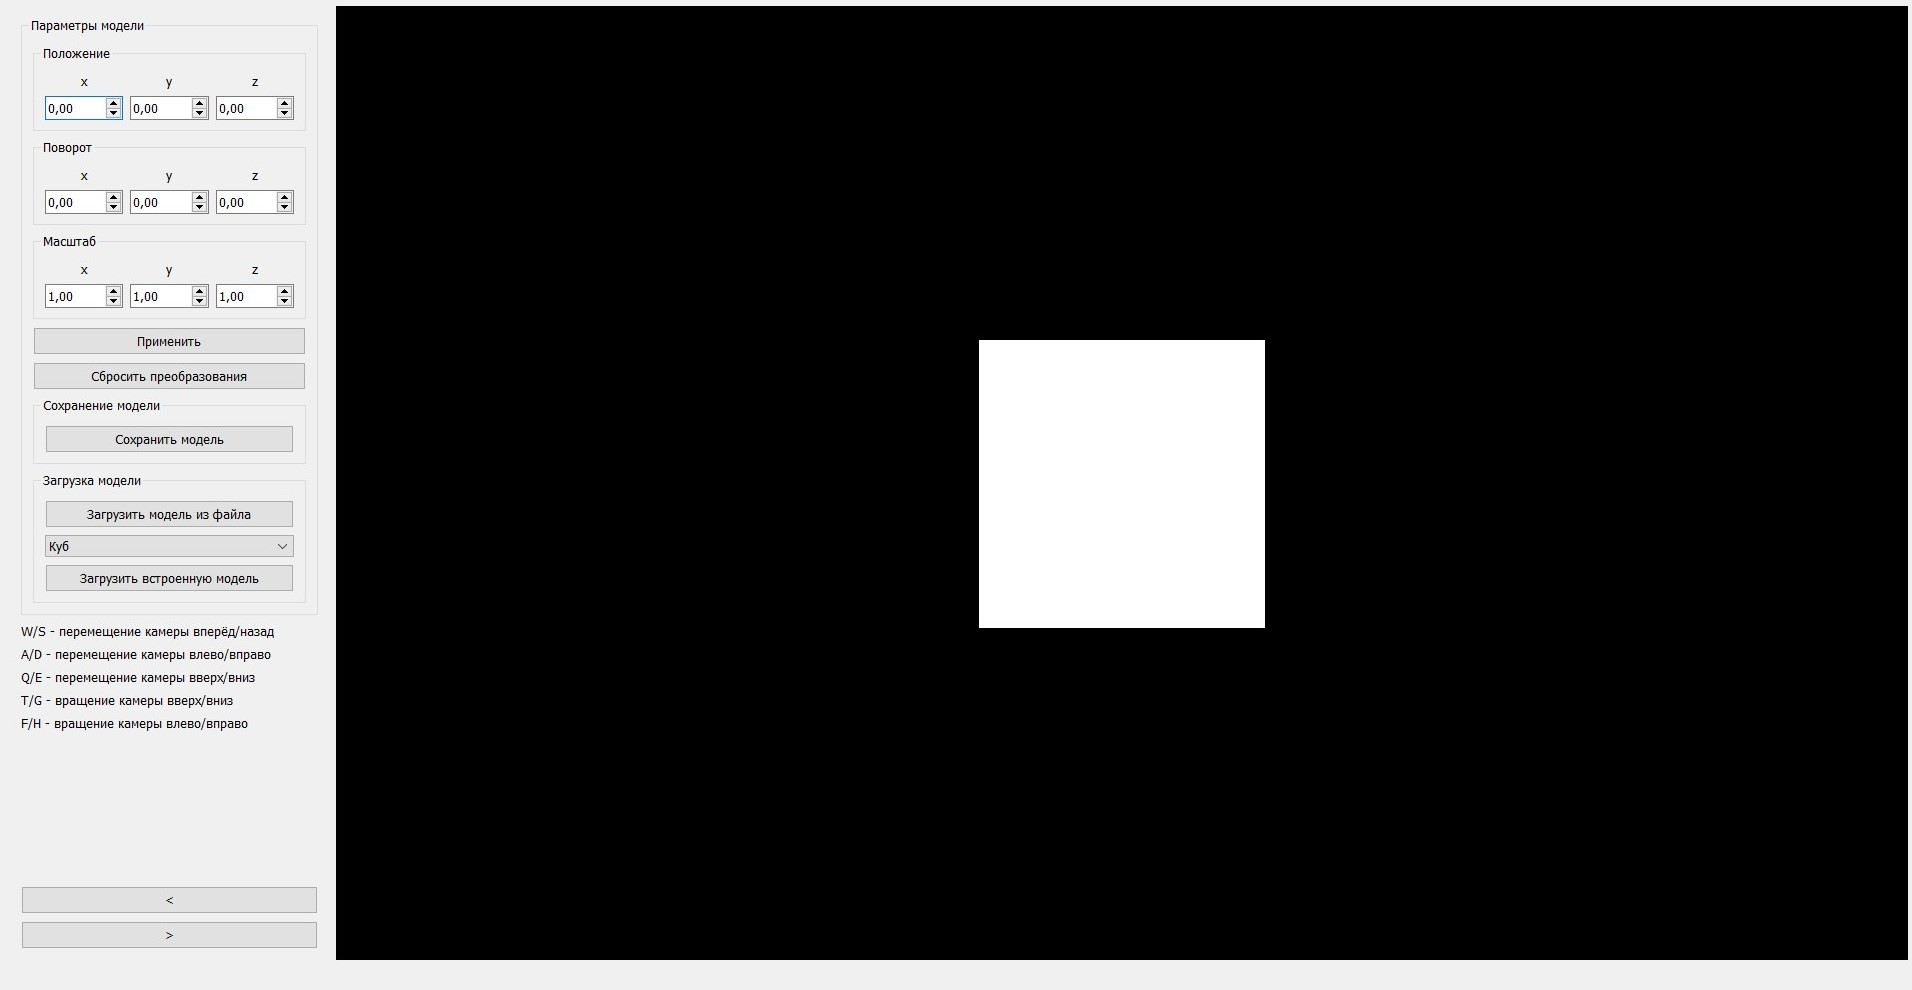
\includegraphics[scale=0.25]{qt_test_1}}
	\caption{Окно, содержащее интерфейс работы с моделью}
	\label{fig:qt_test_1}
\end{figure}

Произвёдем тестирование фукнции загрузки файла из модели. Для этого загрузим модель тора из файла. Ниже на рисунках \ref{fig:qt_test_2}---\ref{fig:qt_test_3} представлены интерфейс загрузки файла и результат загрузки модели в программу.

\begin{figure}[H]
	\center{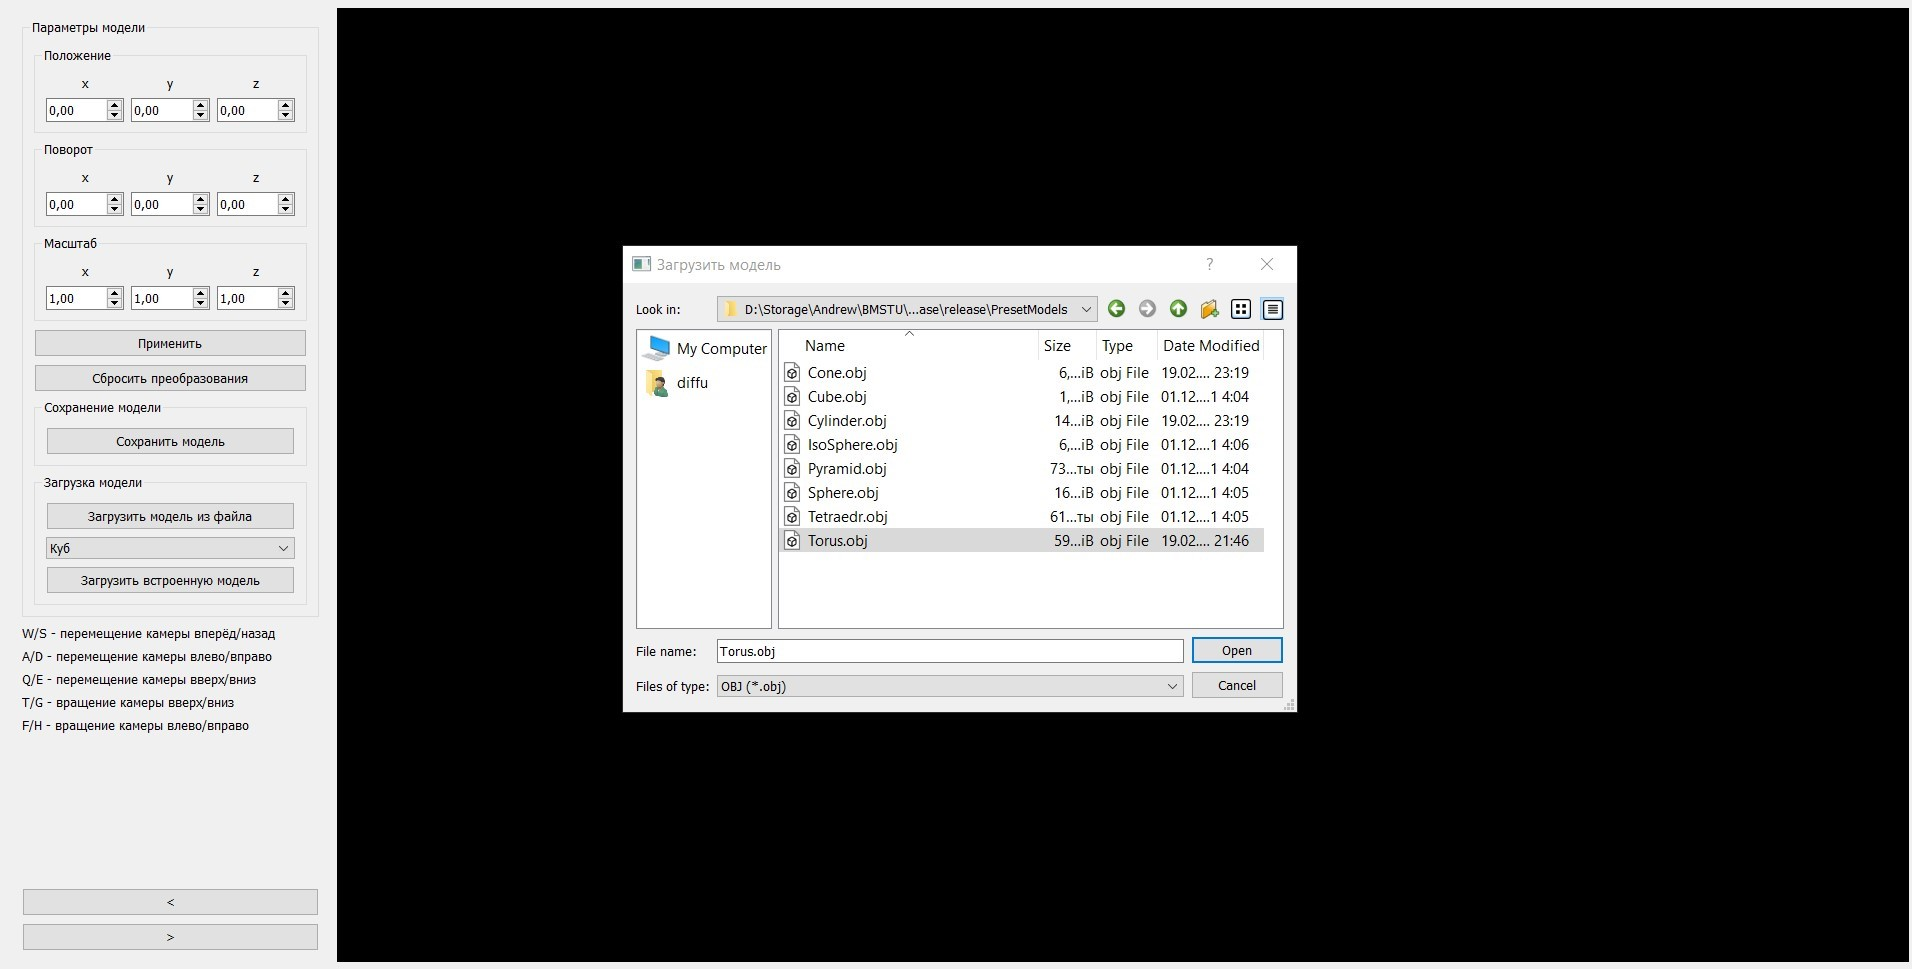
\includegraphics[scale=0.25]{qt_test_2}}
	\caption{Интерфейс загрузки файла}
	\label{fig:qt_test_2}
\end{figure}

\begin{figure}[H]
	\center{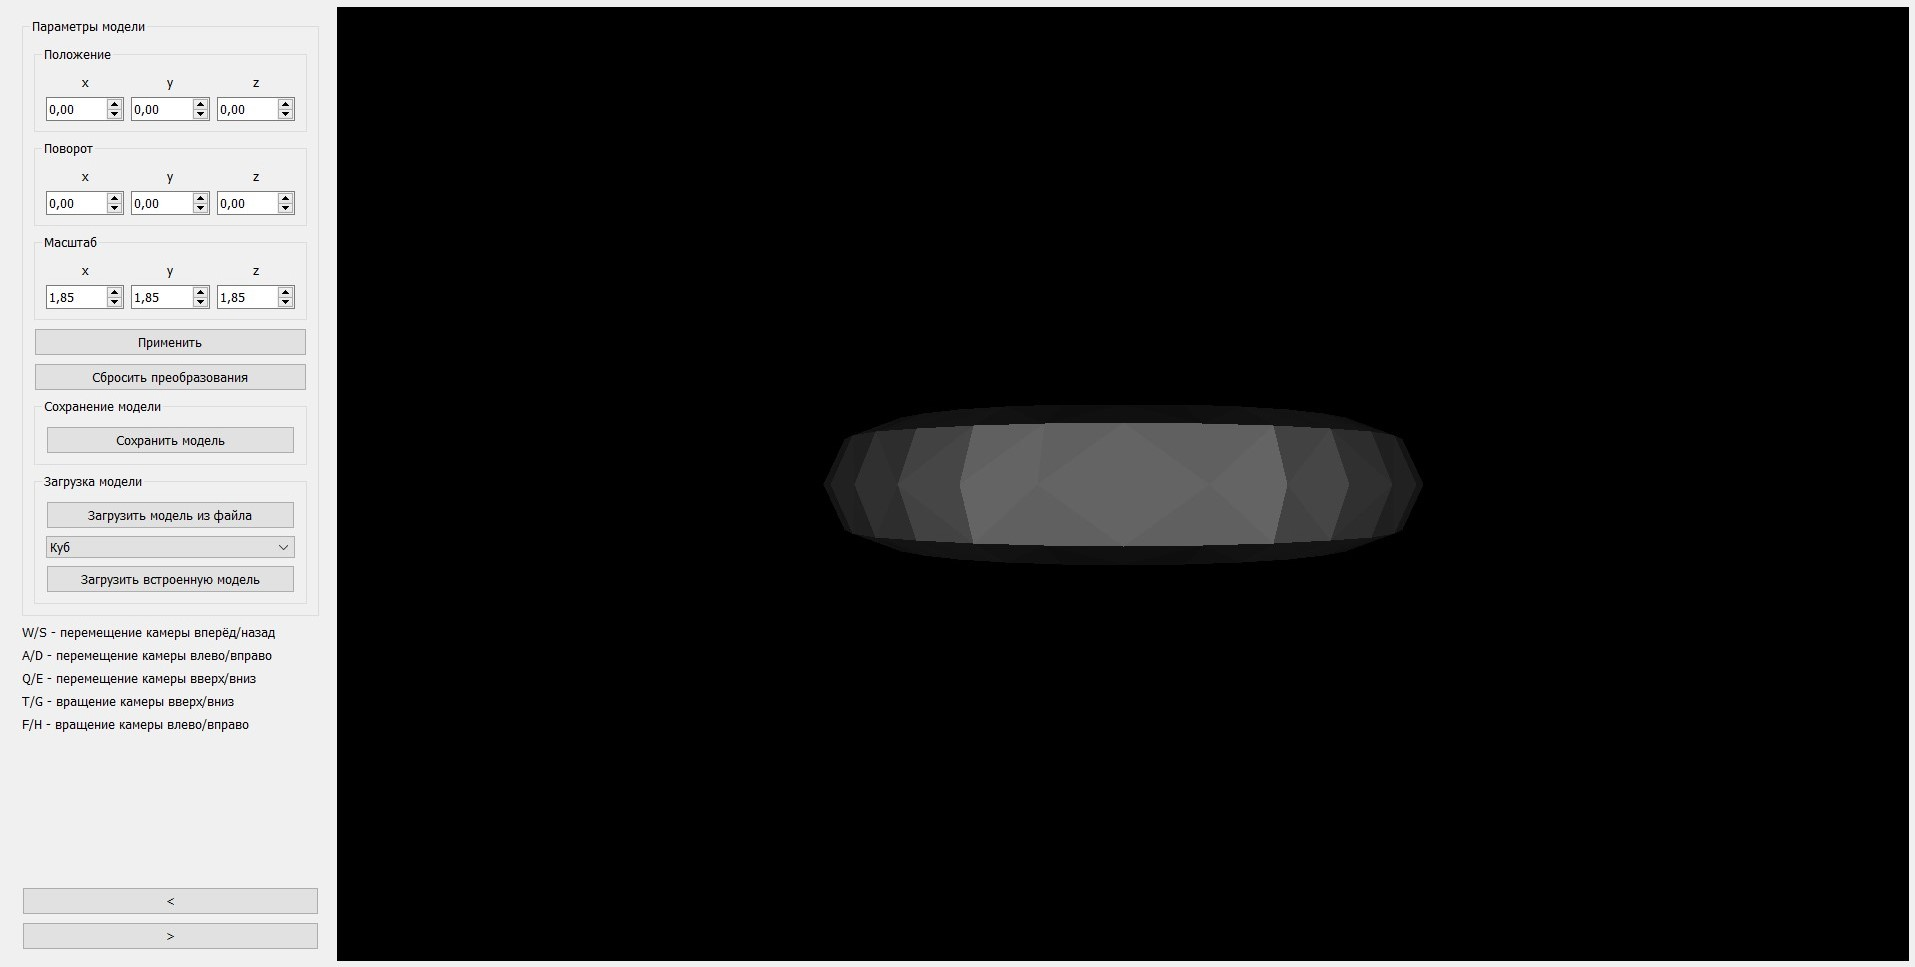
\includegraphics[scale=0.25]{qt_test_3}}
	\caption{Загруженная на сцену модель тора}
	\label{fig:qt_test_3}
\end{figure}

Произведём тестирование функции сохранения снимка модели в виде файла с изображением. Ниже на рисунках \ref{fig:qt_test_4}---\ref{fig:qt_test_6} представлены интерфейс сохранения снимка и полученный снимок.

\begin{figure}[H]
	\center{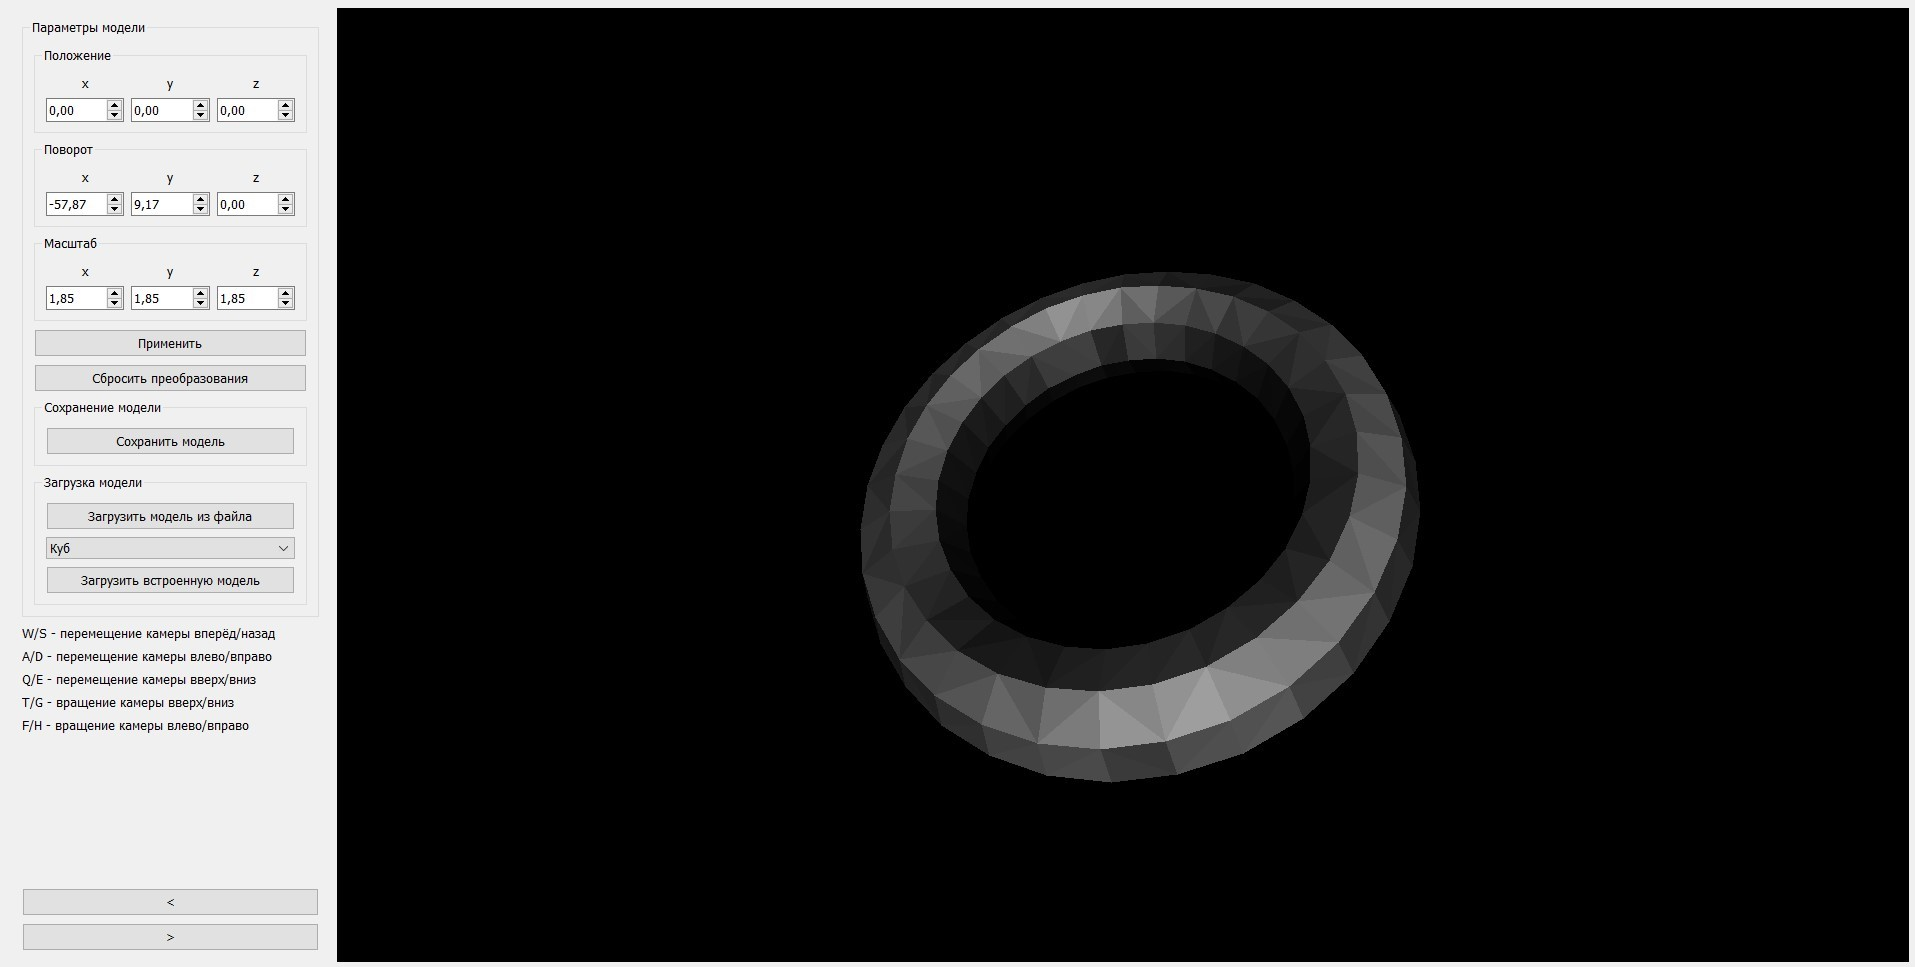
\includegraphics[scale=0.25]{qt_test_4}}
	\caption{Вид сцены, который будет записан в снимок}
	\label{fig:qt_test_4}
\end{figure}

\begin{figure}[H]
	\center{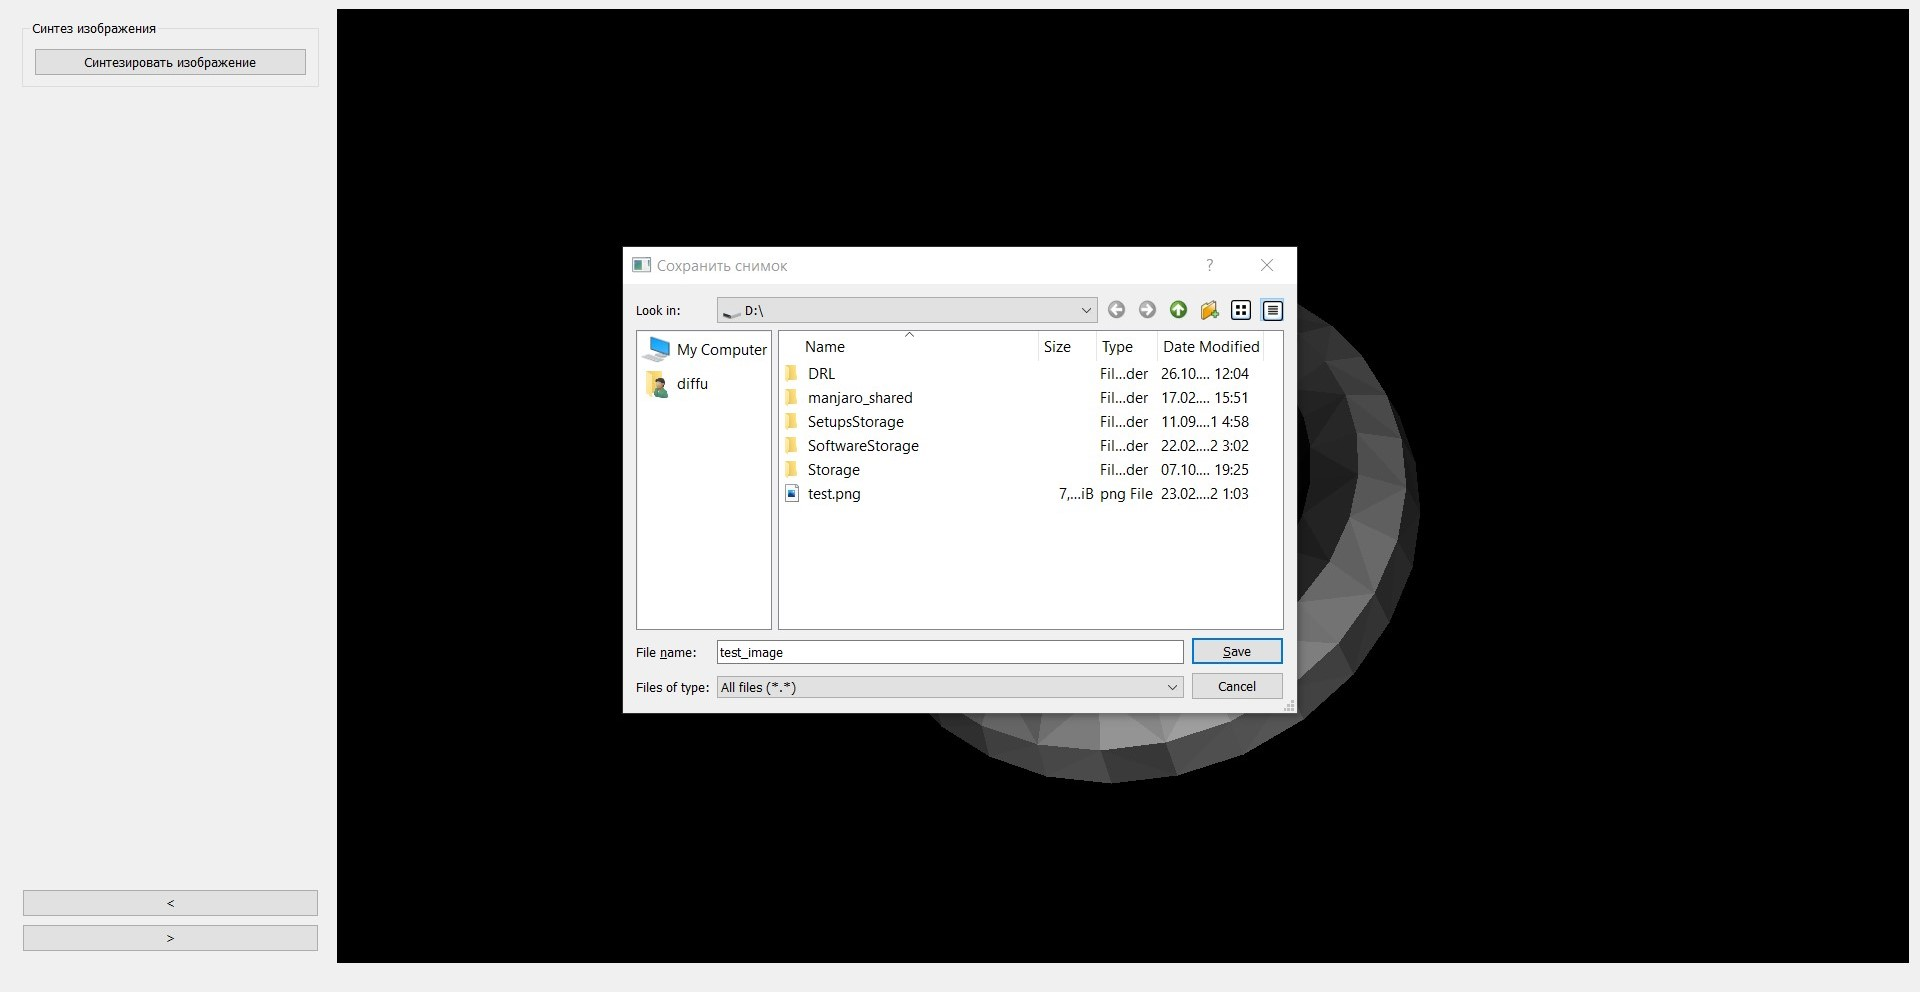
\includegraphics[scale=0.25]{qt_test_5}}
	\caption{Интерфейс сохранения снимка}
	\label{fig:qt_test_5}
\end{figure}

\begin{figure}[H]
	\center{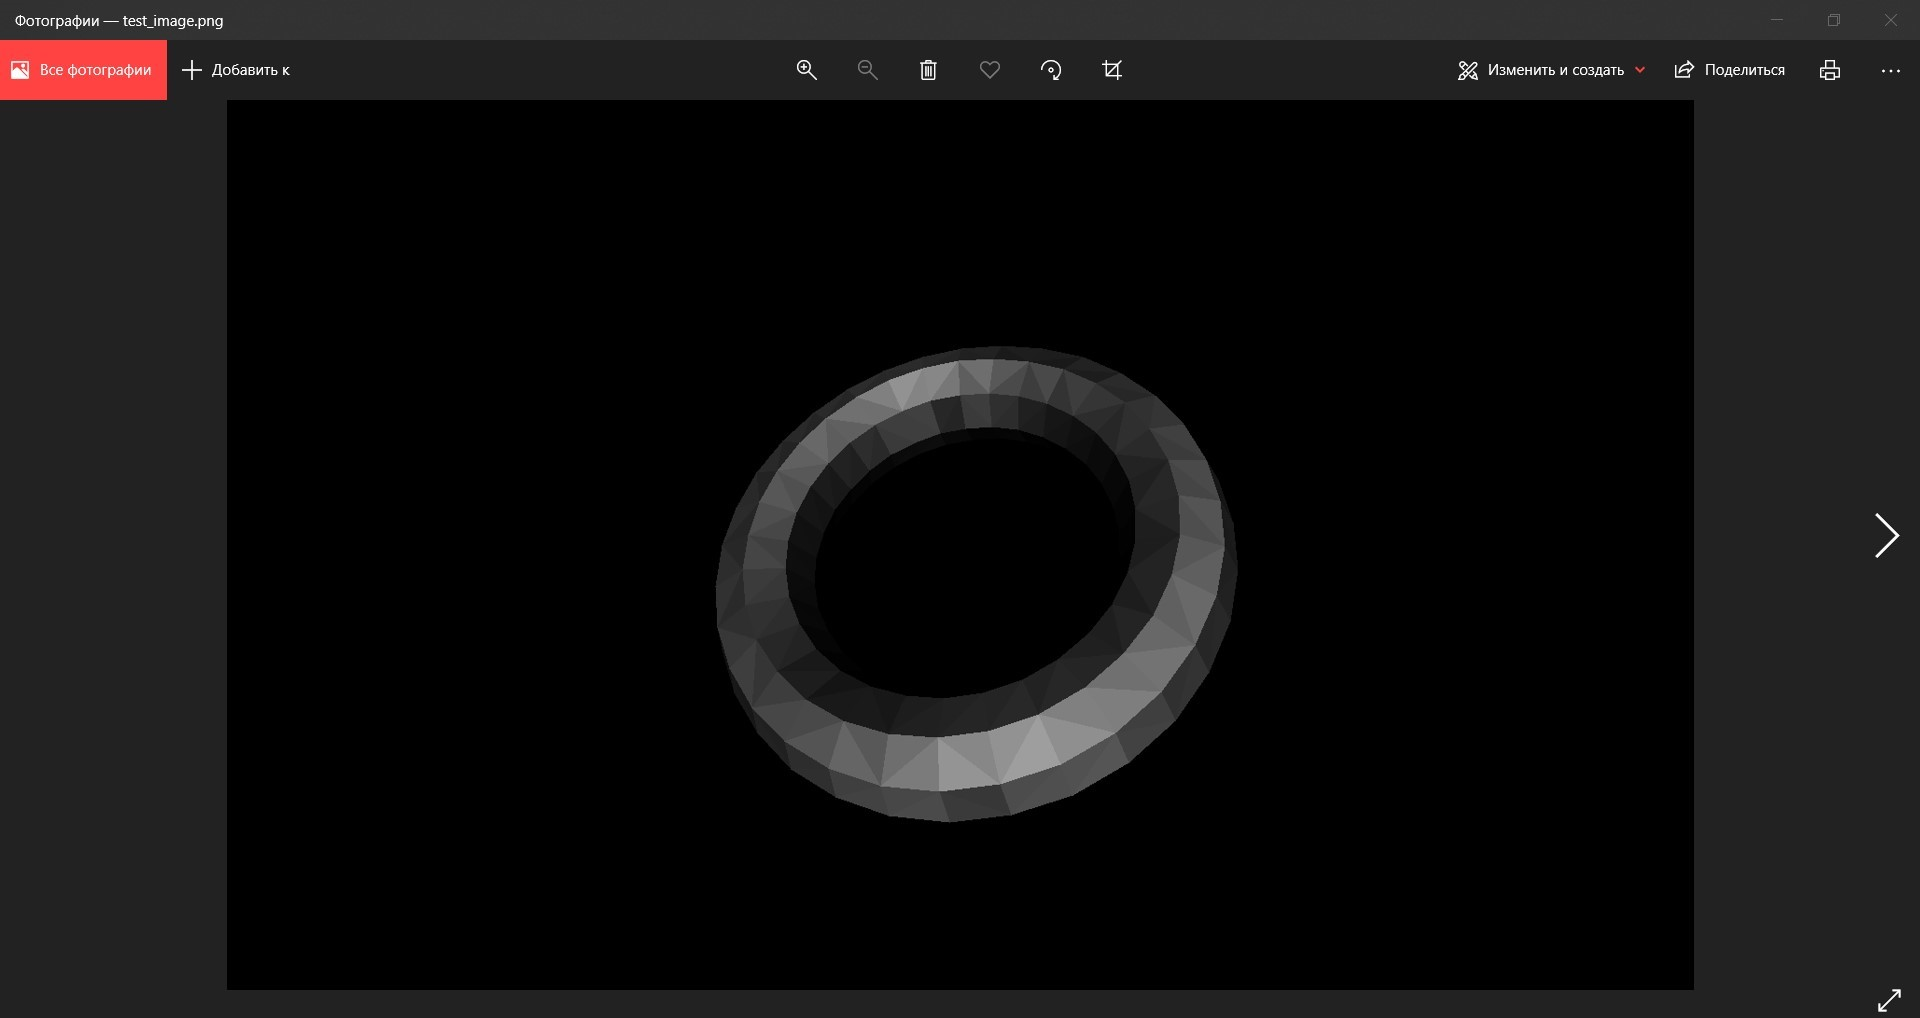
\includegraphics[scale=0.25]{qt_test_6}}
	\caption{Сохранённый снимок}
	\label{fig:qt_test_6}
\end{figure}

Произведём тестирование функции нахождения модели из списка, наиболее подходящей к модели, изображённой на снимке. Ниже на рисунках \ref{fig:qt_test_8}---\ref{fig:qt_test_9} представлены интерфейс загрузки снимка и модель, которая была подобрана в результате работы алгоритма. В качестве снимка использовалось изображение \label{fig:qt_test_6}, полученное при тестировании функции сохранения снимка.

\begin{figure}[H]
	\center{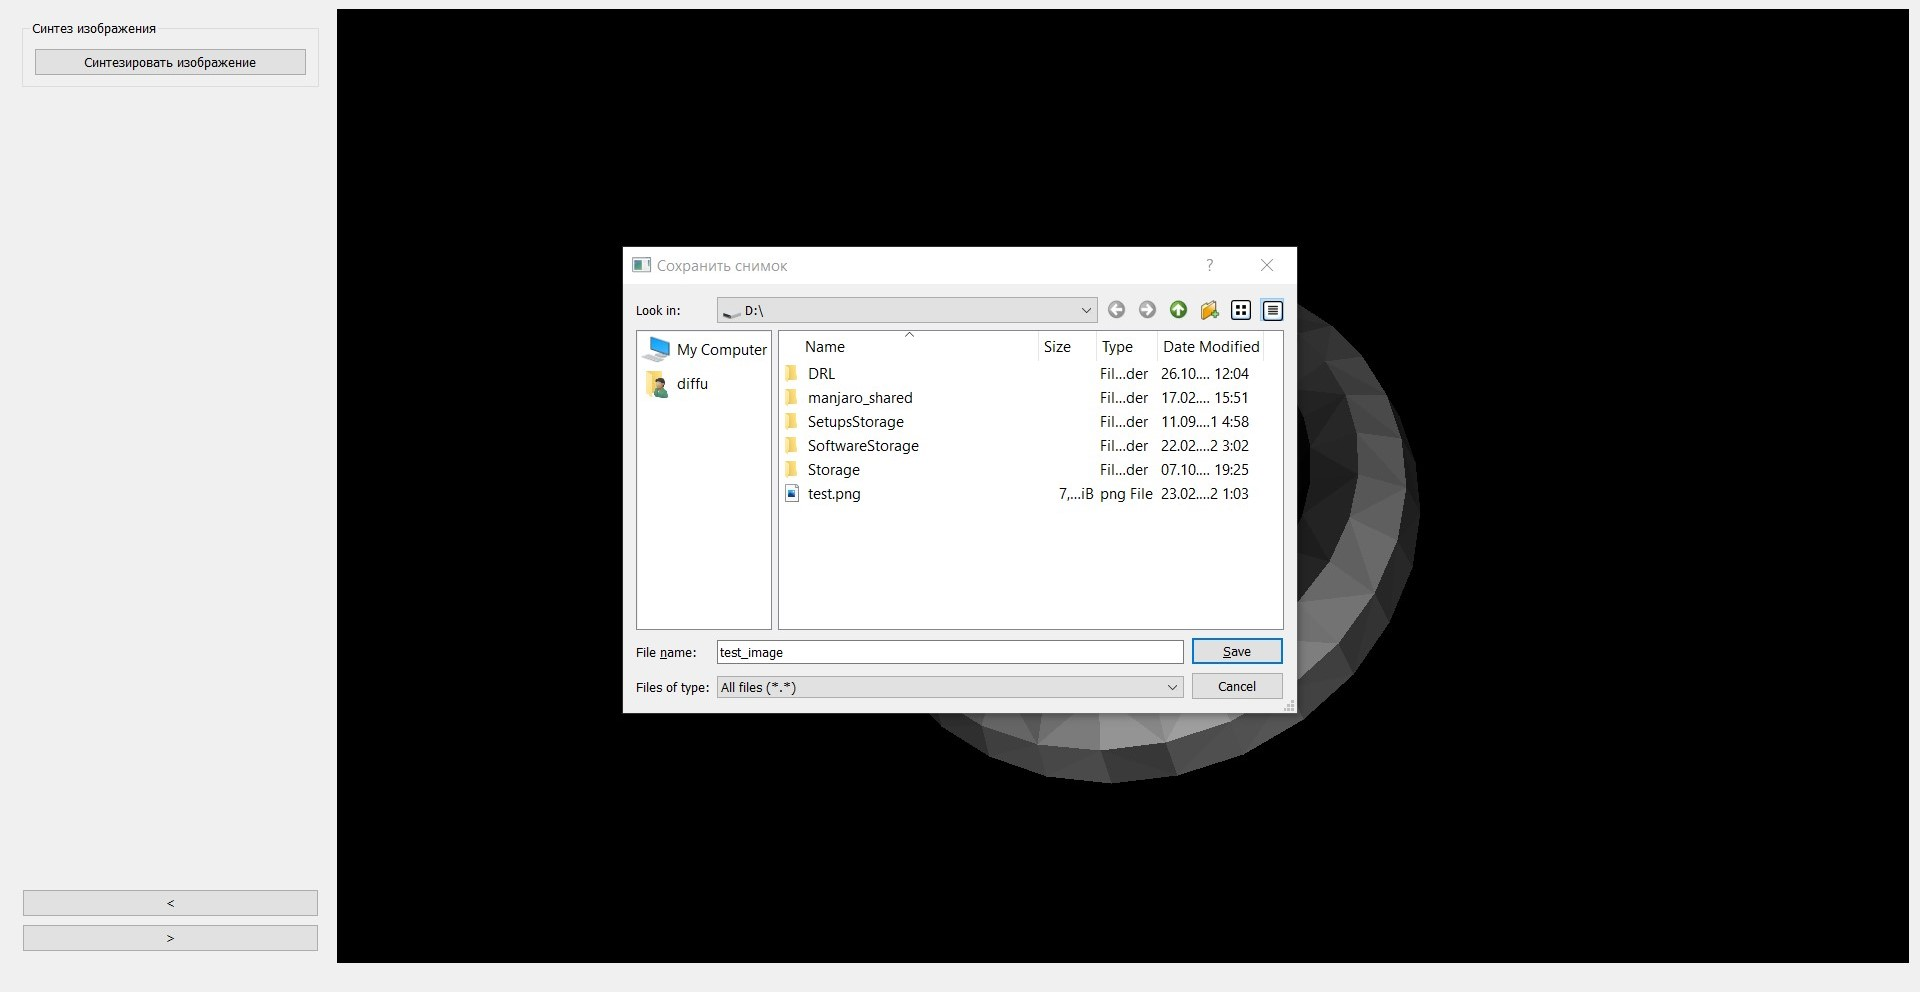
\includegraphics[scale=0.25]{qt_test_5}}
	\caption{Интерфейс загрузки снимка}
	\label{fig:qt_test_5}
\end{figure}

\begin{figure}[H]
	\center{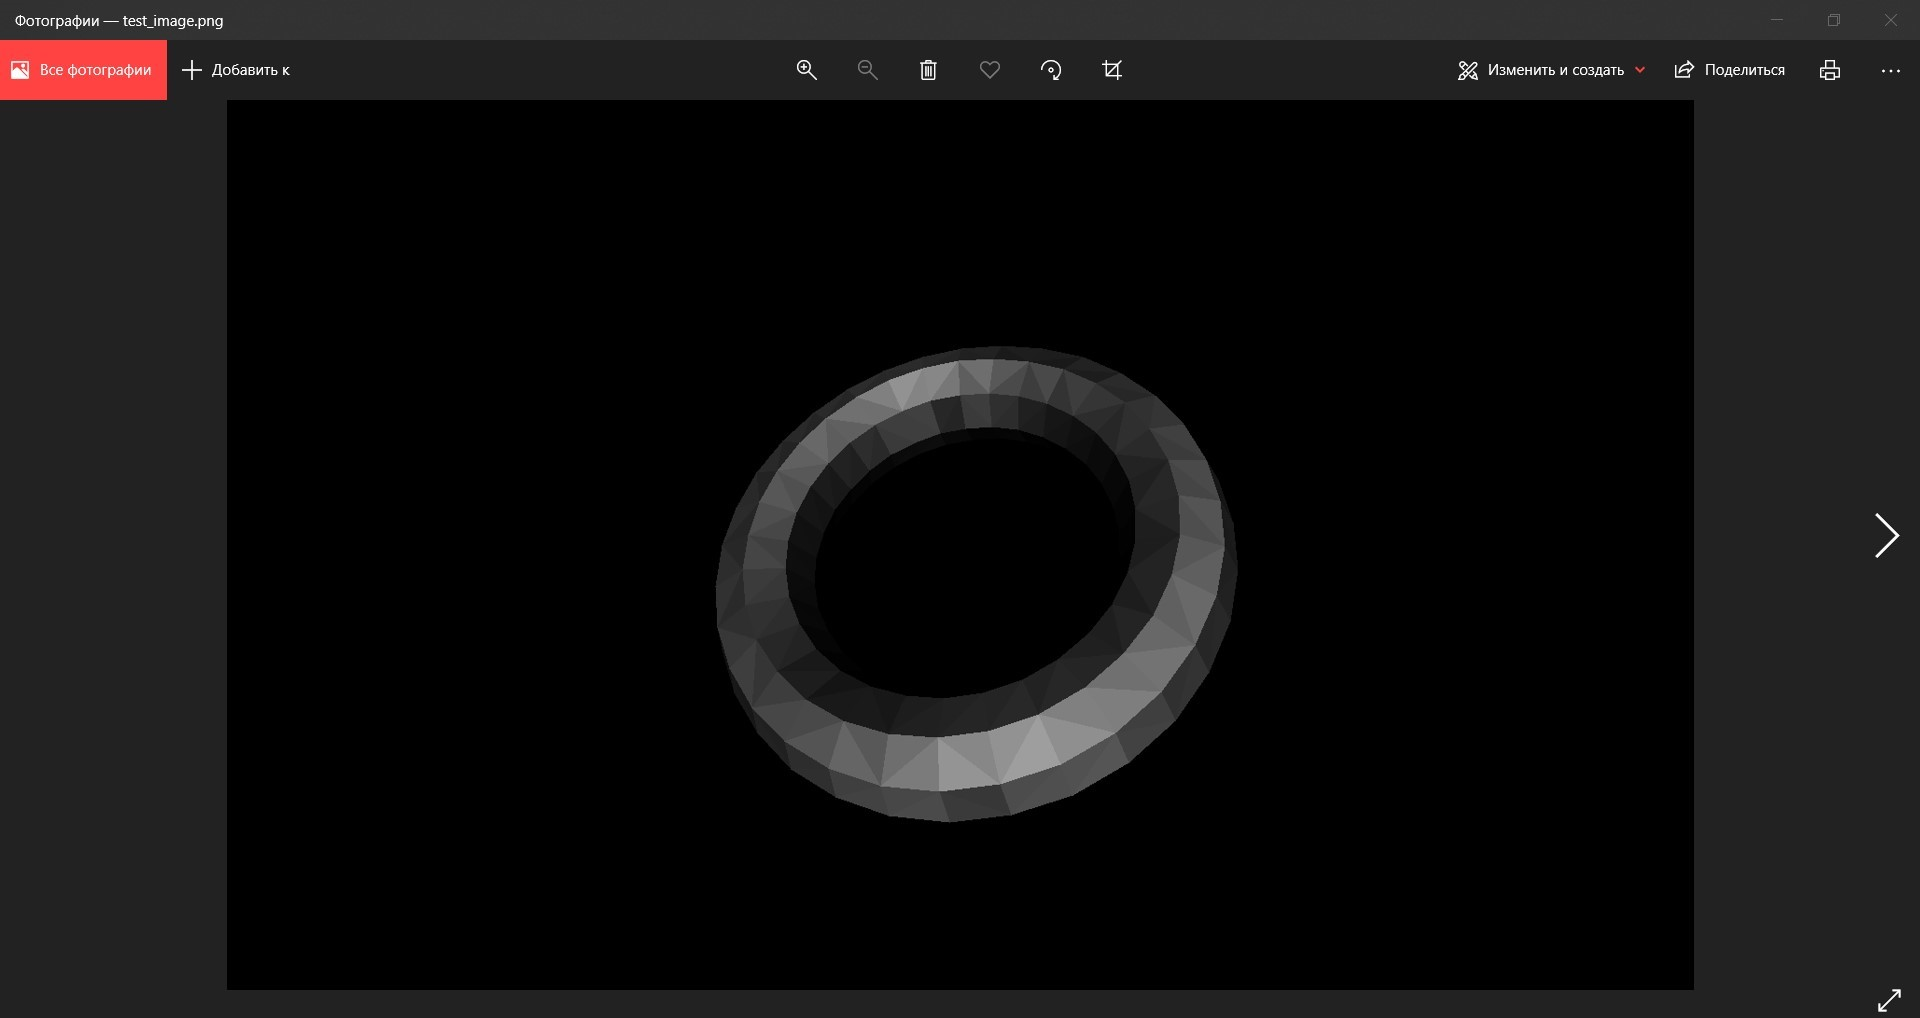
\includegraphics[scale=0.25]{qt_test_6}}
	\caption{Модель, подобранная в результате работы алгоритма}
	\label{fig:qt_test_6}
\end{figure}

\section{Исследование зависимости скорости работы программы от количества полигонов в загружаемой модели}
Целью эксперимента является исследование зависимости скорости работы алгоритма отрисовки от количества полигонов в просматриваемой модели.

Для получения результатов исследовалось изображение сферы, у которой количество полигонов принимало значения от 20 до 1280.

Результаты эксперимента представлены ниже в таблице \ref{tab:res_1} и на графике \ref{fig:exp_1_res}.

\begin{table}[H]
  \begin{center}
    \captionsetup{justification=raggedright}
     \caption{Время отрисовки в зависимости от количества полигонов}
    \label{tab:res_1}
    \begin{tabular}{c|c}
      \textbf{количество полигонов} & \textbf{время отрисовки (нс)}\\
	20 & 80491760.0\\
	40 & 76552860.0\\
	80 & 72199800.0\\
	160 & 64196280.0\\
	320 & 61207200.0\\
	720 & 52398480.0\\
	1280 & 48407940.0\\
      \hline	
    \end{tabular}
  \end{center}
\end{table}

\begin{figure}[H]
	\center{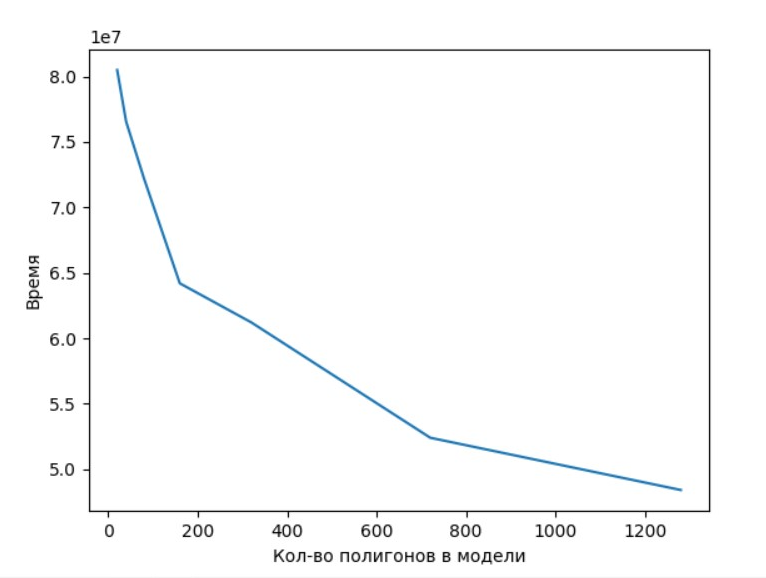
\includegraphics[scale=0.8]{exp_1_res}}
	\caption{Визуализация результатов эксперимента}
	\label{fig:exp_1_res}
\end{figure}

Из полученных результатов можно сделать о вывод о том, что при увеличении количества полигонов время отрисовки изображения уменьшается.

\section{Исследование зависимости скорости работы программы от размера области, которую занимает полигон на экране}
Целью эксперимента являлось исследование зависимости работы алгоритма отрисовки от размера полигона. 

Для получения результатов исследовалась скорость отрисовки полигона, который мастабировался так, что площадь покрытия экрана его проекцией изменялась от 0.5\% до 32\%.

Результаты эксперимента представлены ниже в таблице \ref{tab:res_2} и на графике \ref{fig:exp_2_res}.

\begin{table}[H]
  \begin{center}
    \captionsetup{justification=raggedright}
     \caption{Время отрисовки в зависимости от размера полигона}
    \label{tab:res_2}
    \begin{tabular}{c|c}
      \textbf{размер полигона} & \textbf{время отрисовки (нс)}\\
	0.5\% & 4993100.0\\
	2.0\% & 6198600.0\\
	4.5\% & 8392840.0\\
	8.0\% & 11199080.0\\
	12.5\% & 15184980.0\\
	18.0\% & 19407080.0\\
	24.5\% & 24007740.0\\
	32.0\% & 30205220.0\\
      \hline	
    \end{tabular}
  \end{center}
\end{table}

\begin{figure}[H]
	\center{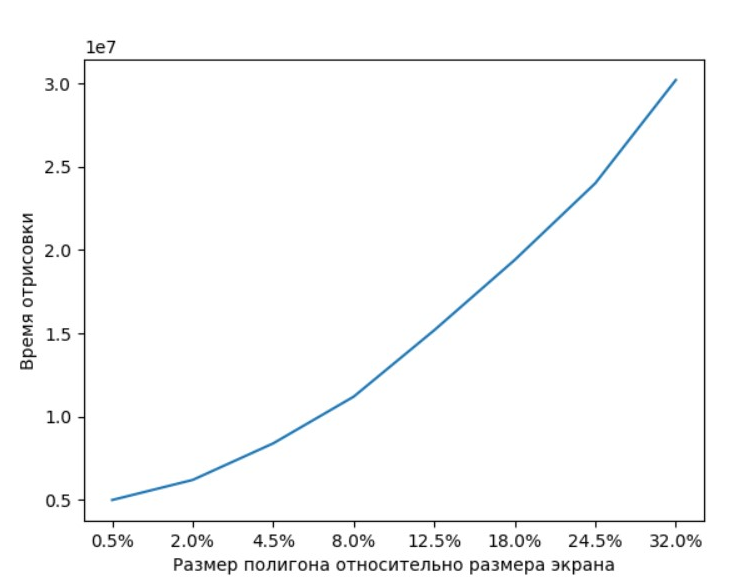
\includegraphics[scale=0.8]{exp_2_res}}
	\caption{Визуализация результатов эксперимента}
	\label{fig:exp_2_res}
\end{figure}


\section{Исследование эффективности работы разработанного алгоритма определения трёхмерного объекта, наиболее вероятно являющимся объектом изображённым на снимке}
Целью эксперимента является оценка эффективности работы разработанного алгоритма определения трёхмерного объекта, наиболее вероятно являющимся объектом изображённым на снимке.

В данном эксперименте создавался набор из 5 снимков для каждого из объектов из списка объектов, после чего данные снимки подаются на вход алгоритму. Полученный объект сравнивается с тем, который служил основой для снимка.

Результаты эксперимента представлены ниже в таблице 

\begin{table}[H]
  \begin{center}
    \captionsetup{justification=raggedright}
     \caption{Соотношение количества корректно определённых результатов к количеству некорректно определённых результатов для каждого из рассматриваемых трёхмерных объектов}
    \label{tab:res_1}
    \begin{tabular}{c|c}
      \textbf{трёхмерный объект} & \textbf{корректно распознанные из пяти}\\
	куб & 0\\
	тетраэдр & 5\\
	пирамида & 4\\
	сфера & 5\\
	изосфера & 5\\
	тор & 5\\
	цилиндр & 5\\
	конус & 5\\
      \hline	
    \end{tabular}
  \end{center}
\end{table}

Из полученных результатов можно сделать вывод о том, что алгоритм корректно распознаёт объекты, имеющие отличающуюся внешнюю форму, такие как тор, конус, циллиндр, изосферу и сферу. Однако если объекты имеют похожую геометрию, то алгоритм не во всех случаях может определить корректную модель, что происходит в случае куба и пирамиды.

\section{Вывод из экспериментального раздела}
В данном разделе были поставлены эксперименты по оценке зависимости скорости работы алгоритма отрисовки от количества полигонов в просматриваемой модели и по оценке эффективности работы разработанного алгоритма определения трёхмерного объекта, наиболее вероятно являющимся объектом изображённым на снимке. 

В результате эксперимента по оценке зависимости скорости работы алгоритма отрисовки от количества полигонов в просматриваемой модели было выявлено, что скорость работы алгоритма отрисовки зависит от количества полигонов так, что чем больше полигонов, тем быстрее работает алгоритм отрисовки, достигая разницы более чем в 1.6 раз.

В результате эксперимента по оценке зависимости скорости работы алгоритма отрисовки от размера полигонов было выявлено, что скорость работы алгоритма отрисовки зависит от количества полигонов так, что чем больше размер проекции полигона на экран, тем медленнее работает алгоритм, достигая разницы в более чем в 7.5 раз.

В результате эксперимента по оценке эффективности работы разработанного алгоритма определения трёхмерного объекта, наиболее вероятно являющимся объектом изображённым на снимке было выявлено, что алгоритм корректно распознаёт объекты, имеющие заметно отличающуюся внешнюю форму, такие как тор, конус, циллиндр, изосфера и сфера. Однако если объекты имеют похожую геометрию, то алгоритм не во всех случаях может определить корректную модель, что происходит в случае куба и пирамиды.

